% !TEX encoding = UTF-8 Unicode
\documentclass[12pt]{article}
\usepackage{amsmath}
\usepackage{graphicx}
\usepackage{hyperref}
\usepackage[utf8]{inputenc}

\author{Michael Kiefer}
\title{Calculations for the Clean-Air UVC device}

\begin{document}
\maketitle{}

\section{Concept}
We consider a set-up with air flowing through a cylinder, assuming the flow is independent of the position in the cylinder. At the center of the cylinder, we have the UVC lamp (a fluorescent tube). 
We want to calculate the energy that gets deposited on a virus particle while passing through the cylinder. The worst case is a virus passing at the wall of the cylinder, with the greatest distance to the lamp.

At that position, we have an Irradiance $I$ as
\begin{equation}
I   = \frac{E}{A_{\text{surface}}},  \label{eqn:irradiance}
\end{equation}
with the Energy $E$ and the side surface of the cylinder $A_{\text{surface}}$,

The outer surface of the tube is determined by the length $l$ and the radius $r$ of the tube as

\begin{equation}
A_{\text{surface}} = 2\pi r l.  \label{eqn:surface}
\end{equation}

The energy is determined by the power $P$ emitted by the lamps within the time $t$ that it takes for a volume element to pass through the irradiated part of the tube

\begin{equation}
E = P  t  \label{eqn:energy}
\end{equation}

We derive the time from the air flow $\Phi$, the volume $V$ that passes through the tube in a given time.
\begin{align}
\Phi &= V / t\\
\Rightarrow t &=V / \Phi
\end{align}

The volume is given by the geometry of the cylinder, using length and base area $A_{\text{base}}$
\footnote{we do not use the cylinder's radius fo calculating the area here, as we want to keep it for the generalization in section \ref{sect:multitube}.}
\begin{equation}
V = l A_{\text{base}} \label{eqn:volume}
\end{equation}

With equations \eqref{eqn:energy}, \eqref{eqn:volume} and \eqref{eqn:surface} in \eqref{eqn:irradiance}, we obtain
\begin{equation}
I =\frac{P }{\Phi } \frac{A_{\text{base}}}{2 \pi r }\label{eqn:irradiance_final}
\end{equation}


\section{Multiple lamps}\label{sect:multitube}
We want to estimate the irradiance created by multiple lamps at a certain position in our setup. At such a position, we can calculate the irradiance $I_i $ caused by each of the lamps $i$ with \eqref{eqn:irradiance_final} using the distance to the lamp as $r_{i}$. The resulting irradiance is simply the sum of these\footnote{$P$ in this case is the sum of the powers of the individual lamps $P_i$.}.
\begin{equation}
I_{\text{total}}=  \sum_{i} I_i = \frac{P A_{\text{base}}}{\Phi 2 \pi}  \sum_{i} \frac{1}{ r_i }
\end{equation}

In order to disable the virus particles, we need to expose them to a certain level of irradiation. With this targeted value $I_{\text{target}}$ given, we can calculate the maximum flow $\Phi_{\text{max}}$ that our device can process as

\begin{equation}
\Phi_{\text{max}}=  \frac{P A_{\text{base}}}{I_{\text{target}} 2 \pi}  \sum_{i} \frac{1}{ r_i }
\end{equation}

\section{Application to the MaibornWolff clean air device}

\begin{figure}
   \centering
   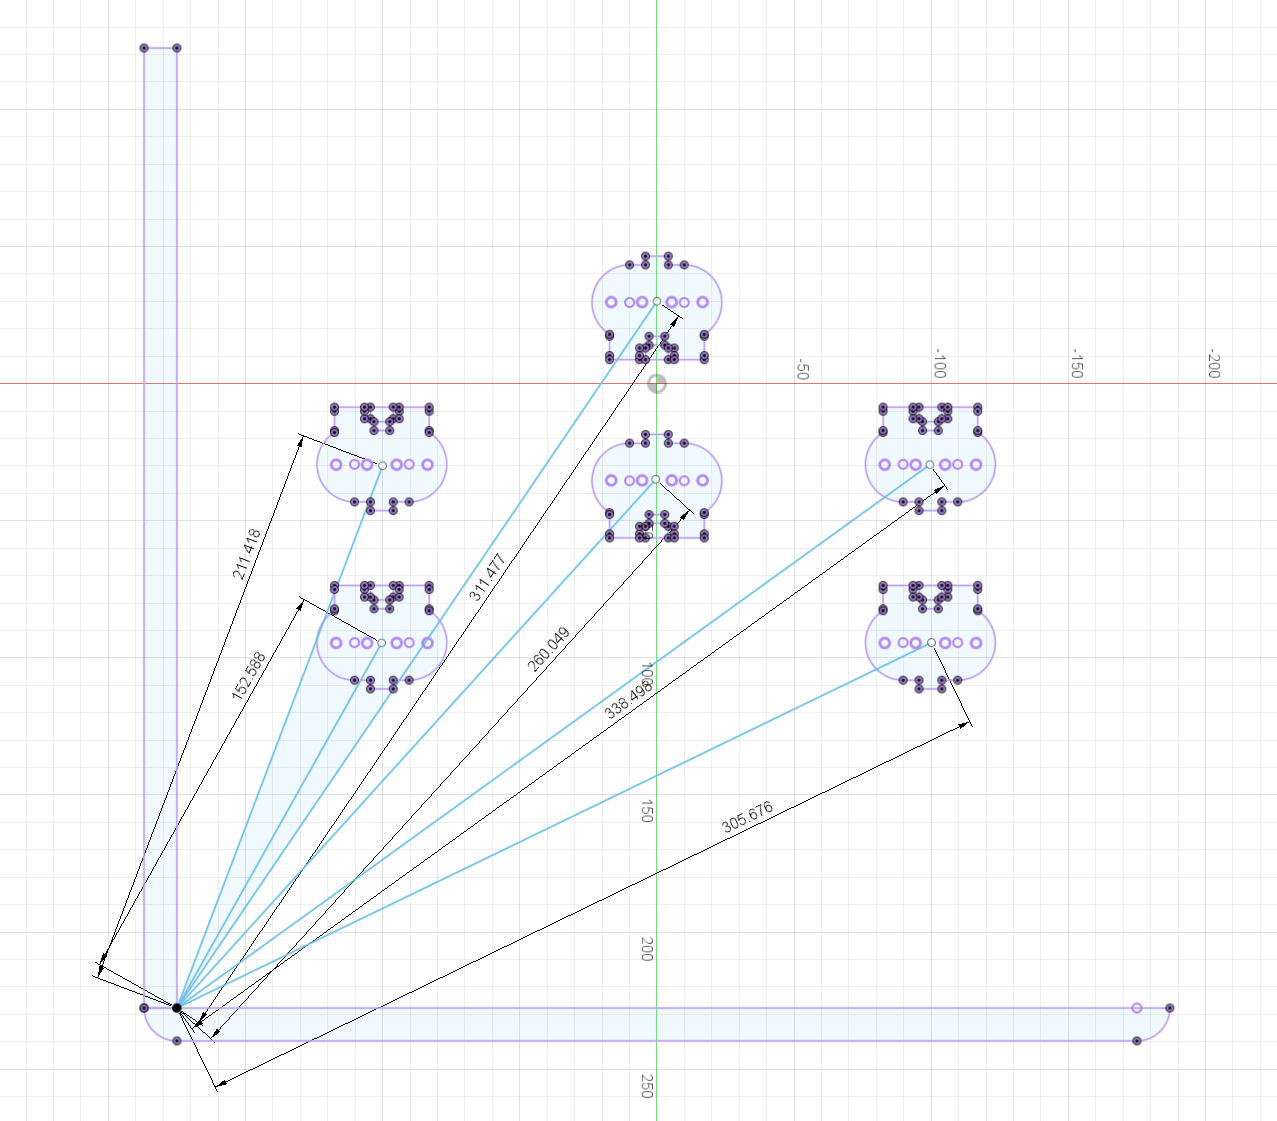
\includegraphics[width=0.45\linewidth]{images/PosA.png} % requires the graphicx package
   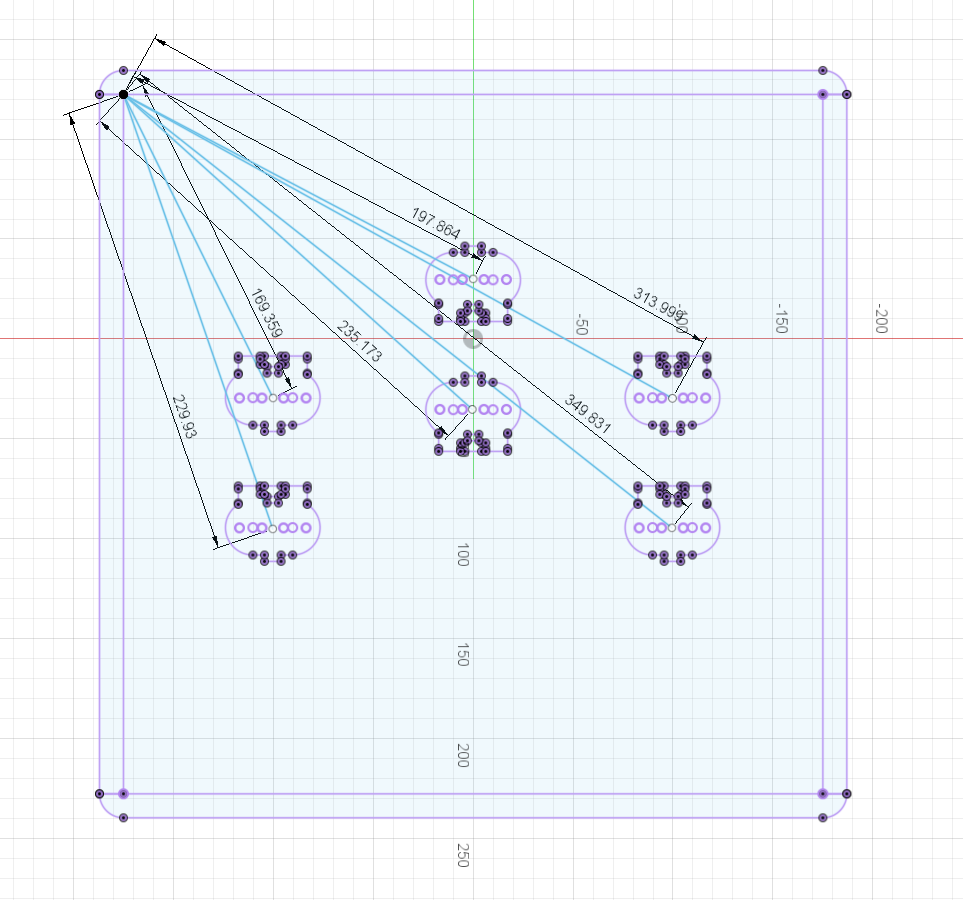
\includegraphics[width=0.45\linewidth]{images/PosB.png} % requires the graphicx package
   \caption{Distances at position A (left) and B (right)}
   \label{fig:distances}
\end{figure}

Numbers on the irradiation dose vary. 
In order to deactivate coronavirus particles, \cite {ozog}  says that an irradiation of 10 J/m$^2$ is sufficient. However, \cite{bianco} says that an irradiation of 37 J/m$^2$ is needed. In \cite{hessling} this value is given as the probable value for the log-reduction dose which would mean that such an irradiation would at least deactivate 90\% of the virus particles. For the ongoing calculation, we aim at an irradiation with 120 J/m$^2$ which would mean a log-3 reduction in case of the number given by \cite{hessling}.

In our set-up, the lamps each consume 36W in electrical power and emit 12W of UVC light.

The two sets of distances given in figure \ref{fig:distances} describe the positions that are furthest away from the lamps and thus the places where the irradiation is the weakest.

Using the excel sheet attached in the source repository, we calculate that the maximum throughput the device can tend to is in the range of 1000 m$^3$/h.


\section{Single lamp, cylindrical appliance}\label{sect:multitube}

For a single-lamp cylindrical setup (now with the base surface as $2\pi r$), equation \eqref{eqn:irradiance_final}
turns into
\begin{equation} 
I  = \frac{P r}{2 \Phi} \label{eqn:irradiance_single}
\end{equation}

The length of the tube has no direct influence on the irradiance! Instead, only the relation between air flow and tube power is important. The fact that the irradiance grows with the radius is only counter-intuitive at first sight.  

Checking the units in \eqref{eqn:irradiance_single}

\begin{align}
  [I]  &= \frac{J/s * m }{ m^3 / s }\\
    &= \frac{J}{m^2}
\end{align}


\begin{thebibliography}{9}

\bibitem{hessling}
   Heßling, Martin et al. 
   “Ultraviolet irradiation doses for coronavirus inactivation - review and analysis of coronavirus photoinactivation studies.”
   GMS hygiene and infection control vol. 15 Doc08. 
   14 May. 2020, 
   doi: https://doi.org/10.3205/dgkh000343
   
\bibitem{bianco}
  Andrea Bianco et al.,
  "UV-C irradiation is highly effective in inactivating and inhibiting SARS-CoV-2 replication"
  medRxiv 2020.06.05.20123463
  doi: https://doi.org/10.1101/2020.06.05.20123463 
  
\bibitem{ozog}
  David M. Ozog, et al.,
  The Effect of Ultraviolet C Radiation Against SARS-CoV-2 Inoculated N95 Respirators
  medRxiv 2020.05.31.20118588; doi: https://doi.org/10.1101/2020.05.31.20118588 
\end{thebibliography}

\end{document}



